\documentclass[a4paper,10pt]{article}
\usepackage[english]{babel}
\usepackage[utf8]{inputenc}
\usepackage{url}
\usepackage[margin=1in]{geometry}
\usepackage{enumitem}

\usepackage[nottoc]{tocbibind}
\usepackage{fancyvrb} 
\usepackage{float}
\usepackage{graphicx}
\usepackage{subcaption}
\usepackage{color}
\usepackage{booktabs}
\usepackage{listings}


\usepackage{subcaption}
\usepackage{graphicx}


\title{Combinatorial Optimization\\Homework 5 – 3SAT Genetic Algorithm}
\author{Matyáš Skalický\\skalimat@fit.cvut.cz}

\begin{document}
\maketitle
\tableofcontents
\medskip

\section{Experiment Setting}
The problem of finding a solution to the boolean formula is called boolean satisfiability problem (SAT). In this homework, we are trying so solve a special class of SAT called \emph{Weighted 3SAT}. In 3SAT, the boolean problem is presented in a conjunctive normal form where all clauses contain exactly three literals. Since the problem is weighted, we are trying to come up with a solution that satisfies the boolean formula while maximizing the sum of weights for the literals that are assigned as true.

To make the measurements fair across different population sizes (further, we also call the population a batch), each experiment is ran for \emph{$3$ seconds} of the CPU time. It is possible that for some settings, the SAT problem isn't solved in this time.

The homework was programmed in Python. To speed-up the computation, as many computations as possible were implemented as vectorized numpy operation. Also, the experiments were ran in parallel on a server with $40$ cores to make the experiments feasible.

\section{Genetic Algorithm}

The implemented genetic algorithm solver is parametrized mainly by 4 hyperparameters:

\begin{description}
	\item[mutation rate]{Probability of randomly flipping a literal's value.}
	\item[batch size]{Size of the population.}
	\item[init type]{How each individual is initialized.}
	\item[fitness type]{Which fitness function is used.}
\end{description}

Generally speaking, we first randomly spawn a pool of instances. Before the CPU time runs out, we repeatedly take a batch of parent instances, and by using selection, recombination and mutation, we create a pool of children of the same size. The detailed steps are described below.

\subsection{Fitness}

Fitness should ideally copy the value of the function which we want to optimize. In case of weighted 3SAT, we are working with 2 objectives which we want to accomplish:

\begin{itemize}
	\item Find a binary assignment that solves the boolean formula.
	\item Maximize the weights of the selected literals.
\end{itemize}

Solving 3SAT is very different from solving the knapsack problem. In knapsack problem, it is trivial to find a feasible solution. Most of the work is then done in optimizing the contents of the bag. In 3SAT, finding any feasible instance is contrary to the knapsack problem very hard. Finding the instance with the highest sum of literal weights further increases the complexity of finding the solution.

In a sense, we operate in 2 modes. In the first mode, we don't know any solution to the 3SAT problem. In the second mode, we have found the solution, but we need to improve the assignment of the literals in order to maximize the weights.

Figuring out the fitness score in genetic algorithms is one of the hardest tasks. First, how do we \emph{push} the algorithm towards solving the SAT problem? And then, how do we design the fitness score in order to keep improving? I have designed two experimental fitness score methods:

\begin{description}
	\item[sum or nothing] Fitness score is $0$ if the solution isn't feasible. Otherwise, it represents the sum of the literals which are assigned true.
	\item[correct count] If current assignment solves the problem, use the sum of weights of the true literals. If it isn't solved, count how many clauses are correctly solved. This helps early on, when no solution was found.
\end{description}

\subsection{Random Initialization}

I've implemented 2 initialization strategies for instance initialization.

\begin{description}
	\item[all false] All literals are initialized as false. This is not an optimal initialization strategy for genetic algorithms as the initial diversity is just non-existent and all of the variation must be introduced by mutation.
	\item[uniform] Randomly select value of each literal. My hypothesis is, that this will be a better initialization strategy than \emph{all false}.
\end{description}


\subsection{Selection}

Selection takes a pool (batch) of candidates on the input. It calculates the total fitness and uses the roulette wheel selection to find the pairs of candidates that go into recombination.

\subsection{Recombination}

We take 2 input instances (\emph{parents}). A single-point crossover is used to create 2 children. If any of the children is valid (fitness is non-0), we return the better child. Otherwise, the better parent is returned.

\subsection{Mutation}

Mutation is controlled by the \emph{mutation\_rate} hyperparameter. It is called on the instances that come out of recombination before we add them into children pool. We randomly flip the value assigned to the literal with the probability defined by the \emph{mutation\_rate}.

\section{Experiments}

As described above, we are running each experiment for $2$ seconds of the CPU time to make different batch sizes comparable. Small batches will be much faster, but there will be less diversity in the population. Large batches will contain diverse initialization pools (depending on the init strategy), but the processing will be much slower.

\subsection{Pilot Experiments}

During the pilot experiments, we would like to determine the ideal combination of hyperparameters (batch size, mutation rate, initialization strategy and fitness function) to solve the weighted 3SAT problem. My hypothesis is, that the uniform (random) initialization will work better than setting all instances as false. Also I assume that the the fitness function which considers the count of correctly assigned clauses should perform significantly better as it pushes the genetic algorithm towards improvements rather than blindly guessing and mutating before a feasible solution is found.

Pilot experiments were performed on subsample of $100$ instances for maximum runtime of $3$ seconds. Although the genetic algorithm is randomized, we can assume that the aggregate results should have sufficient statistical power.

\begin{figure}[!htb]
\centering
\begin{subfigure}{.49\linewidth}
    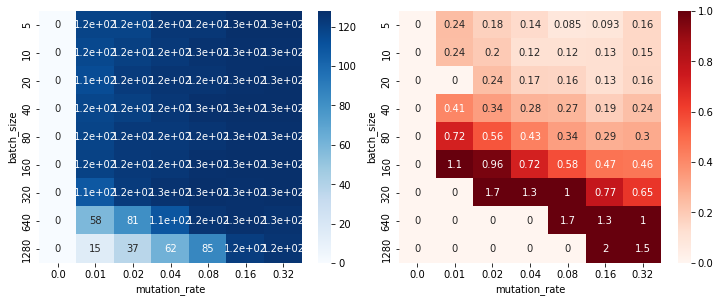
\includegraphics[width=\linewidth]{images/pilot_allfalse_correct_count.png}
    \caption{all-false init, correct count fitness func.}
\end{subfigure}
\begin{subfigure}{.49\linewidth}
    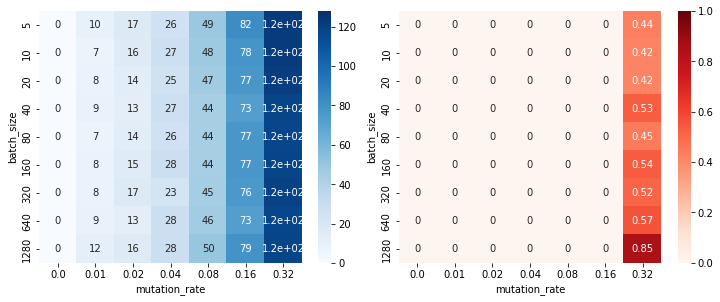
\includegraphics[width=\linewidth]{images/pilot_allfalse_sum_or_nothing.png}
    \caption{all-false init, sum or nothing fitness func.}
\end{subfigure}
\hfill
\begin{subfigure}{.49\linewidth}
    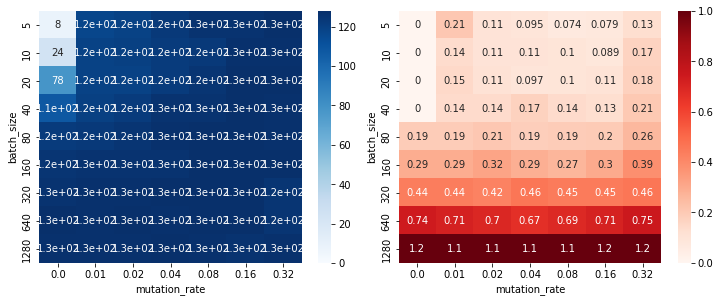
\includegraphics[width=\linewidth]{images/pilot_uniform_correct_count.png}
    \caption{uniform init, correct count fitness func.}
\end{subfigure}
\begin{subfigure}{.49\linewidth}
    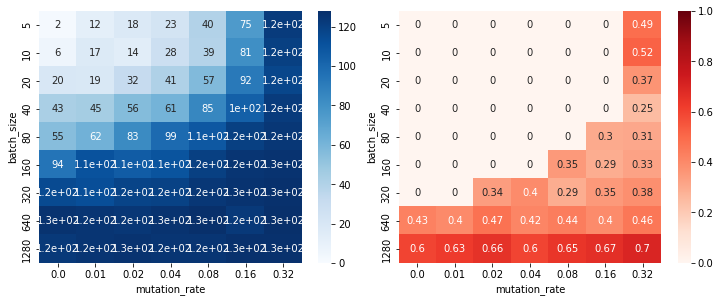
\includegraphics[width=\linewidth]{images/pilot_uniform_sum_or_nothing.png}
    \caption{uniform init, sum or nothing fitness func.}
\end{subfigure}        
\caption{Pilot experiments on the \lstinline{wuf20-78-N1} dataset. Left side contains number of successfully solved 3SAT instances out of 100 with maximum of 3s CPU runtime. Right side shows mean runtime until the instance was solved.}
\label{fig:small:pilot}
\end{figure}

Results of the pilot experiments can be seen in the Figure \ref{fig:small:pilot}. As expected, we can see that the genetic algorithms benefit from the initial variability of random initialization. In general, the correct count fitness function led to a more stable behavior and more successfully solved instances.

We can see, that for the correct-count fitness function, the best settings are when the batch size is relatively small ($20$) and mutation fairly large ($8\%$).

\begin{figure}[!htb]
    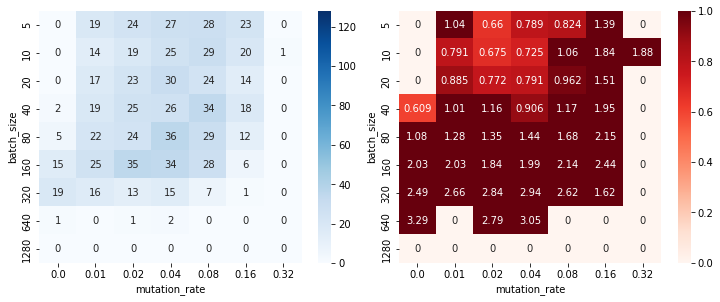
\includegraphics[width=\linewidth]{images/pilot_medium_uniform_correct_count.png}
    \caption{Dataset \lstinline{wuf50-0931}. Correct count fitness function with uniform initialization. Maximum 3s runtime. Left side shows number of solved instances, right mean runtime before the instance was solved.}
    \label{fig:pilot:mid}
\end{figure}

For the dataset with larger instances (\lstinline{wuf50-0931}), we are going to see the results for the best combination mentioned above. Results can be seen in the figure \ref{fig:pilot:mid}. Compared to the smaller dataset, more bigger instances profited from larger batch size, but overall, the hyperparameter setting of $8\%$ mutation and batch size of $40$ still holds.


%For a knapsack problem, the ideal setting was a small mutation rate (around 3\%) and a moderate batch size. 

% As described before, the naive initialization produces very sparse bags. With very low mutation rate, there isn't enough diversity in the initial population pool to achieve good performance. As we can see in the Figure \ref{pilot_naive}, a small mutation rate is required. Interesting finding is that we are able to solve the problem even with a very small batch size. Even though the batch size is very small, the algorithm will be very fast. And it is able to go through many iterations before the time runs out.

\subsection{Detailed Experiment}

After selecting the hyperparameters, we are going to observe how the algorithm performs through different generations.

\begin{figure}[!htb]
    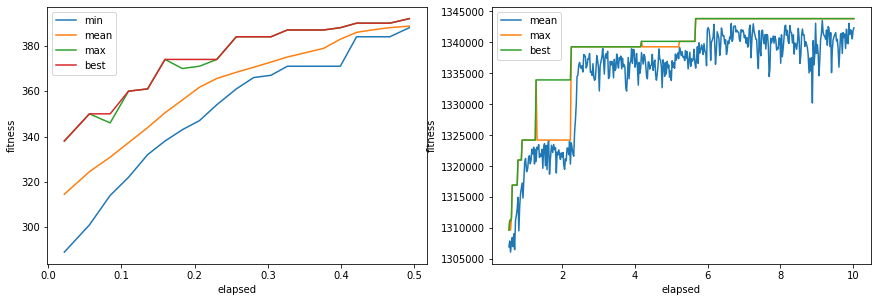
\includegraphics[width=\linewidth]{images/medium_side_by_side.png}
    \caption{Example from dataset \lstinline{wuf50-201-N1}. Correct count fitness function with uniform initialization. Left side shows the fitness before the solution is found. Right after the solution was found.}
    \label{fig:example:runtime:sidebyside}
\end{figure}

Example run is shown in the figure \ref{fig:example:runtime:sidebyside}. We can immediately see how the optimization performs in different optimization modes - before the solution was found (left), the fitness score progresses as better solutions are rewarded better scores. On the right, we can see the same optimization problem after a solution was found. Since we use the weighted sum of all of the correct clauses.

It is worth noting, that the improvements after a solution was found are rather sparse. This of course highly depends on the weighting of the individual clauses as the algorithm can get stuck in a local minima easily.

\section{Discussion and Takeoffs}

Fifth homework (and also the fourth) was much more fun compared to the previous ones. Genetic algorithms are one of my favorite black-box methods and even though I've implemented them several times, I still had fun applying it on the knapsack problem and now on the 3SAT.

To make the solution as fast as possible, I have tried to write as many computations as vectorized numpy matrix multiplications. This has ensured that the runtime would be feasible. For the pilot experiments, I ran them in parallel on a 40-core server to get to the results faster.

Compared to the knapsack problem where finding a solution is trivial, from my perspective, genetic algorithms seem less usable for weighted 3SAT. They are effective at finding a solution, but it is difficult to design a fitness function that motivates the algorithm to learn before, and also after a feasible solution was found. But finding the best proxy function is perhaps always the most challenging part on implementing genetic algorithms.

\end{document}